\documentclass{hw}
\usepackage{xcolor}

% STUDENTS: Please fill these out with your information
\newcommand{\name}{Matthew Shen}
\newcommand{\netid}{mds377}
\newcommand{\collaborators}{Linjing Rao(lr534)}
% / STUDENT

\newcommand{\hwnum}{1}
\newcommand{\duedate}{September 26, 11:59pm ET}
\renewcommand{\title}{Stable Matching, Greedy, Divide and Conquer}

\newcommand{\submission}{\textbf{Submission.}}

\newtheorem{claim}{Claim}

\begin{document}

%%%%%%%%%%%%%%%%%%%%%%%%%%%%%%%%%%%%%%%%%%%%%%%%%%%%%%%%%%%%%%%%%%%%%%%%%%%%%%%%
% Problem 1: G-S algorithm

\begin{problem}
    Your friend is wrapping up medical school and applying for residency programs, but is concerned and confused about how the matching system works. As the local expert on algorithms, your colleague wants your help understanding how matchings work. 

    \begin{subproblem}
        (\textit{2 points})
        Your friend tried to implement the textbook Gale-Shapley (G-S) algorithm in Python. We provide this code in the homework materials in \texttt{problem\_1/p1\_a.py}. Using this implementation, your friend thinks they found a way to propose a ranking that unfairly advantages them in getting the school of their choice.
        
        There is a logical bug in the implementation. Provide a minimal test case demonstrating the bug, i.e., an input with the smallest possible $n$ that, when run with the buggy implementation, outputs a non-stable matching. Write your test case input in \texttt{problem\_1/p1a\_test.txt}.  
    \end{subproblem}

    \begin{subproblem}
        (\textit{8 points})
        Now we turn to characterizing the performance of
        this implementation. Fix the bug from part (a) and conduct an 
        of the implementation (see homework instructions
        in the first page). Include the fixed code in \texttt{problem\_1/p1\_b.py}.
        
        Provide a brief explanation of the performance you observe, and explain why the implementation does not achieve $\bigO(n^2)$ run time advertised for the G-S algorithm.
    \end{subproblem}

    \begin{solution}
        The environment used for the empirical performance analysis can be seen below:
            \begin{itemize}
                \item CPU: Intel(R) Core(TM) i7-8500Y CPU @ 1.50GHz (4 threads, 4.20GHz)
                \item OS \& Version: Debian GNU/Linux 11 (bullseye)
                \item Memory: 15.53 GB
            \end{itemize}

        The graph created from the empirical performance analysis can be seen below:
            \begin{figure}[h]
                \centering
                    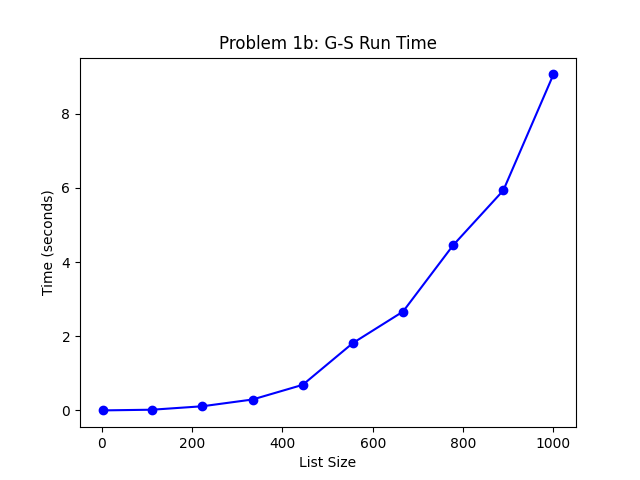
\includegraphics[width=0.5\textwidth]{figures/problem-1b.png}
            \end{figure}

        The following code provided does not reach $\bigO(n^2)$. For the worst case scenario all hospitals have the same preference order for all doctors, and all doctors have the same preference order for all hospital. Additionally, the hospitals list is in the same order as the preferences that all the doctors have; therefore, a stable match is when the hospital number and Doctor number matches (i.e. \{ 0:0, ... , n:n\}).This means, in the first loop through the first hospital gets matched and all other hospitals are not matched. In the second loop the program goes through all the hospitals again except for the first/matched hospital. In the second loop on the second hospital gets matched because all other hospitals want to get the second student, but the second student's top choice is the second hospital. This means we get a loop has a time complexity of $\bigO(n)$ and is run $\bigO(n!)$ times. This means the algorithm is $\bigO(n!)$.  
    \end{solution}

    \begin{subproblem}
        \newcommand{\worstrank}{{\tt wr}}
        (\textit{10 points})
        Correct and improve the run time of the G-S implementation and turn it in for
          auto-grading. It must be correct (always outputting a stable matching) and should run in the expected $\bigO(n^2)$ time. 
          Provide a description of the optimizations you implemented.
          Additionally, provide an empirical performance analysis of your
          implementation in the same environment (same system and configuration) that
          you performed the earlier analysis. Include your new implementation in \texttt{problem\_1/p1\_c.py}.
    \end{subproblem}

    \begin{solution}
        In order to go from $\bigO(n!)$ to $\bigO(n^2)$ there are two changes that need to be made. The first is that in problem-1b the program loops through all the hospitals even if they are matched. This means that hospitals that are already matched are still checked even when they have already been matched to a doctor. This was fixed by setting a list of unmatched hospitals at the start. When a hospital gets matched they are removed from the unmatched hospital list, and it is this list that is continuously looped through until all hospitals are matched. This means a hospital is only looped through if they don't have a match.
        
        The second change is the removal of a doctor from the hospitals preference list if they are already matched to a hospital with a higher ranking. This prevents the program from looping through doctors that we know are matched to their preferred hospital.
        
        These two changes make it so the program only loops through all the doctors once for each hospital. Each of these operations is $\bigO(n)$ so the total time complexity is $\bigO(n^2)$.
    
        For the empirical performance analysis the environment was:
        \begin{itemize}
            \item CPU: Intel(R) Core(TM) i7-8500Y CPU @ 1.50GHz (4 threads, 4.20GHz)
            \item OS \& Version: Debian GNU/Linux 11 (bullseye)
            \item Memory: 15.53 GB
        \end{itemize}
            
        The graph from the empirical performance analysis can be seen below:
        \begin{figure}[ht]
          \centering
              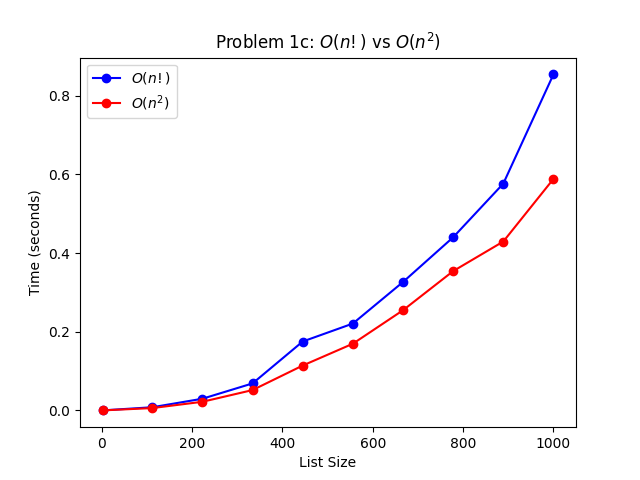
\includegraphics[width=0.5\textwidth]{figures/problem-1c.png}
        \end{figure}
    \end{solution}
\end{problem}

\newpage
%%%%%%%%%%%%%%%%%%%%%%%%%%%%%%%%%%%%%%%%%%%%%%%%%%%%%%%%%%%%%%%%%%%%%%%%%%%%%%%%
% Problem 2

\begin{problem}
    In the {\em interval covering problem}, one is given a time interval $[0,M]$ and a collection of closed subintervals $\mathcal{I} = \{[a_i,b_i] \mid i=1,2,\ldots,n\}$ whose union is $[0,M]$. (Interpret intervals as jobs and, interpret $a_i$ and $b_i$ as the {\em start time} and {\em finish time} of job $[a_i,b_i]$.) The goal is to find a subcollection $\mathcal{J} \subseteq \mathcal{I}$, containing as few intervals as possible, such that the union of the intervals in $\mathcal{J}$ is still equal to $[0,M]$.
    
    You can assume that the numbers $M,a_1,a_2,\ldots,a_n,b_1,b_2,\ldots,b_n$ are all non-negative integers, and that $a_i < b_i$ for all $i$. You should assume that the list of intervals given in the problem input could be arbitrarily ordered; in other words, don't make an assumption that the input to the algorithm presents the intervals
    sorted according to any particular criterion.
    
    (\textit{20 points}) Below we have listed four greedy algorithms for this problem. At least one of them is correct, and at least one is incorrect. For {\em every} incorrect algorithm, provide an example of an input instance such that the algorithm outputs an incorrect answer in your write-up. (Either a set of intervals that fails to cover $[0,M]$, or a set that covers $[0,M]$ but has a greater number of intervals than necessary.) For {\em every} correct algorithm, write, ``The algorithm is correct.'' For {\em at least one} of the correct algorithms, implement the algorithm to run in $O(n \log n)$; that is $\Theta(n \log n)$ or faster. In the write-up, indicate which algorithm you implemented and briefly describe your implementation strategy. Include your implementation in \texttt{problem\_2/p2.py}.
        \begin{subproblem}
            \textbf{Select Latest Finish Time:} Initialize $\mathcal{J}=\emptyset$. Until the intervals in $\mathcal{J}$ cover all of $[0,M]$, repeat the following loop: find the maximum $c \in [0,M]$ such that $[0,c]$ is covered by the intervals in $\mathcal{J}$, or if there is no such $c$ then set $c=0$; of all the intervals containing $c$ select one whose finish time is as late as possible and insert it into $J$.
        \end{subproblem}
    
        \begin{solution}
            The algorithm is correct. This algorithm was implemented. For the implementation we first sort the intervals by start time and then end time. We set up initial variables for the output list and c. We also set two pointer called max\textunderscore val which starts off as the first interval and i which starts off as 0. Next, we loop through all the intervals. If a given interval's start time is less than 0 we look at if it ends after the current max\textunderscore val. If it does end before the current max\textunderscore val we start this as the new max\textunderscore val. Regardless if the interval's start time is less than c we move onto the next interval. If the interval's start time is greater we can append the current max\textunderscore val to the output list and set c to be the end time of the stored max\textunderscore val. This is done because the list is sorted, so once we find a value greater than c we can leave the loop. Finally, we run into an issue with the final value missing from output list. This is solved by appending the final max\textunderscore val to the output list, but a logical is used to stop an append if there is only a single value.
    
            The time complexity of this algorithm is $O(n \log n)$ This is because the list is sorted which has a time complexity of $O(\log n)$ and we loop through each value in the list to determine if it should be added to the covering interval which has a time complexity of $O(n)$. This means the total run time is $O(n \log n)$
        \end{solution}
    
        \begin{subproblem}
            \textbf{Select Longest Interval:} Initialize $\mathcal{J}=\emptyset$. Until the intervals in $\mathcal{J}$ cover all of $[0,M]$, repeat the following loop: among all the intervals in $\mathcal{I}$ that are not already contained in the union of the intervals in $\mathcal{J}$, select one that is as long as possible (i.e., that maximizes $b_i-a_i$) and add it to $\mathcal{J}$.
        \end{subproblem}

        \begin{solution}
            $$
            \mathcal{I} = \{[0_0,8_0], [8_1,9_1], [9_2,10_2], [0_3,5_3], [5_4,10_4]\}, [0,10]
            $$
            $$
            \mathcal{J}_{ans} = \{[0_0,8_0], [8_1,9_1], [9_2,10_2]\}
            $$
            $$
            \mathcal{J}_{opt} = \{[0_3,5_3], [5_4,10_4]\}
            $$
        \end{solution}

        \begin{subproblem}
            \textbf{Delete Earliest Redundant Interval:} Initialize $\mathcal{J}=\mathcal{I}$. While there exists a redundant interval in $\mathcal{J}$ --- one that is contained in the union of the other intervals in $\mathcal{J}$ --- find the redundant interval in $\mathcal{J}$ with the earliest finish time and remove it from $\mathcal{J}$.
        \end{subproblem}

        \begin{solution}
            $$
            \mathcal{I} = \{[0_0,8_0], [8_1,9_1], [9_2,10_2], [0_3,5_3], [5_4,10_4]\}, [0,10]
            $$
            $$
            \mathcal{J}_{ans} = \{[0_0,8_0], [8_1,9_1], [9_2,10_2]\}
            $$
            $$
            \mathcal{J}_{opt} = \{[0_3,5_3], [5_4,10_4]\}
            $$
        \end{solution}
    
        \begin{subproblem}
            \textbf{Delete Latest Redundant Interval:} Initialize $\mathcal{J}=\mathcal{I}$. While there exists a redundant interval in $\mathcal{J}$ --- one that is contained in the union of the other intervals in $\mathcal{J}$ --- find the redundant interval in $\mathcal{J}$ with the latest finish time and remove it from $\mathcal{J}$.
        \end{subproblem}

        \begin{solution}
            This answer is not correct.
            $$
            \mathcal{I} = \{[0_0,8_0],[7_1,10_1],[1_2,4_2],[4_2,7_2]\}, [0,10]
            $$
            $$
            \mathcal{J}_{ans} = \{[7_1,10_1],[1_2,4_2],[4_2,7_2]\}
            $$
            $$
            \mathcal{J}_{opt} = \{[0_0,8_0],[7_1,10_1]\}
            $$
        \end{solution}

    {\bf A note about tie-breaking:} When implementing any of the algorithms above one must choose a tie-breaking rule. In other words, when more than one interval meets the criterion defined in the algorithm specification (such as the latest finishing redundant interval) one must specify which of the eligible intervals is chosen. In the context of this problem, if you are asserting that an algorithm is correct, it should mean that you believe the algorithm gives the correct answer on every input instance {\em no matter how the tie-breaking rule is implemented;} that is what your proof of correctness should show. When you assert an algorithm is incorrect, for full credit you should supply an input instance that leads to an incorrect output {\em no matter how the tie-breaking rule is implemented.} However, significant partial credit will be awarded forproviding an input instance that leads to an incorrect output {\em for some choice of tie-breaking rule}, though not necessarily for every tie-breaking rule.

\end{problem}
\newpage
%%%%%%%%%%%%%%%%%%%%%%%%%%%%%%%%%%%%%%%%%%%%%%%%%%%%%%%%%%%%%%%%%%%%%%%%%%%%%%%%
% Problem 3

\newcommand{\rank}{\textnormal{rank}}
\newcommand{\Colon}{:}
\newcommand{\dotdot}{..}
\newcommand{\numinv}{\textrm{NI}}
\newcommand{\numlargeinv}{\textrm{NLI}}

\begin{problem}
    We consider how to count the number of \emph{large} inversions between two rankings. Consider a set~$N$ with size $n$. 
    A ranking is a 1-1 function $\rank\Colon N \rightarrow [1\dotdot n]$. In other words, $\rank$ maps each item in $N$ to a unique integer, and therefore represents an ordering of the $N$ items where lower integer values indicate higher rankings. 
    
    As described in the Kleinberg-Tardos textbook, Section~5.3, we can compare two rankings, $\rank_i$ and $\rank_j$, by counting the number of inversions. We label each $x \in N$ with $\rank_i(x)$, hence making $\rank_i = [1, \dots ,n]$. Then, we define $\rank_j$ in terms of $\rank_i$ and count the number of inversions in $\rank_j$. 
    
    Suppose now we want to consider large inversions, where we define a threshold $0 < \delta < n$ and let $\numlargeinv_{\delta,i,j}$ equal the number of pairs $x,y \in [1\dotdot n]$ such that $x < y$ and $\rank_j(x) > \rank_j(y) + \delta$. In other words, we only consider inversions large if their ranking differs by at least~$\delta$.
        \begin{subproblem}
            (\textit{6 points})
            Design and implement a $\Theta(n^2)$ algorithm that iterates over every pair of points and determines $\numlargeinv_{\delta,i,j}$ given two rankings $\rank_i$ and $\rank_j$ and a threshold $\delta$. Describe the algorithm in the write-up, and include your implementation in \texttt{problem\_3/p3\_a.py}.
        \end{subproblem}

        \begin{solution}
            To start off we initialize the number of large inversion to 0. Next, we loop through the length of the list provided. This gives us the index of the first value we are looking at ($x$). We then loop through all values after ($x$) to the end of the list. This gives us pairs of ($x,y$) where $x$ will always be less than $y$. Finally, we check to see if $rank_j(x)$ is > $rank_j(y) + \delta$. If this is true then we add one to the number of large inversions we are counting.
            
            This algorithm would run in $O(n^2)$ because we are looping through the list a total of 2 times. Once to set $x$ and once to set $y$.
        \end{solution}

        \begin{subproblem}
            (\textit{14 points})
            Design and implement a $\Theta(n\log n)$ algorithm to calculate $\numlargeinv_{\delta,i,j}$. Include your implementation in \texttt{problem\_3/p3\_b.py} and explain your algorithm in the write-up. Using your local experimental system perform an empirical performance analysis of both implementations (see homework instructions in the first page) and determine for what~$n$ does the asymptotically faster implementation dominates.
        \end{subproblem}

        \begin{solution}
            Please answer here.
        \end{solution}
\end{problem}

\newpage
%%%%%%%%%%%%%%%%%%%%%%%%%%%%%%%%%%%%%%%%%%%%%%%%%%%%%%%%%%%%%%%%%%%%%%%%%%%%%%%%
% Problem 4


\begin{problem}
    Given a sequence of integers $a_1,\ldots,a_n$ we want to find the number of times the most frequent pairwise difference appears. Let $\delta_{i, j} = a_i - a_j$ for $i \ne j$ in the list. Suppose you know one of the \href{https://en.wikipedia.org/wiki/Mode_(statistics)}{modes} (i.e. the most frequent value) of the list of all the $\delta_{i, j}$'s is $\delta_{mode}$. We want to count for how many values $\delta_{i, j} = \delta_{mode}$. 

    \begin{subproblem}
        (\textit{8 points})
        Design and implement a $\Theta(n \log n)$ algorithm that given a sequence of integers $a_1,\ldots,a_n$ and $\delta_{mode}$ as described above, outputs the frequency of $\delta_{mode}$. Include your implementation in \texttt{problem\_4/p4\_a.py}.
    \end{subproblem}
  
    \begin{solution}
        Given that our run time for this problem is $O(n \log n)$ we first sort the values. Next we create a list of tuples that has the number of times a given integer appears. This is done by counting the number of time you see the value in the list and leaving the list once a new value is found. This is done in $O(n)$ time. Finally, we can use a binary search for each value to figure out where the index of the $\delta_{mode}$. We also need to take into account the case where if $\delta_{mode}$ is 0 then we add the frequency minus 1. This is to avoid duplicated a subtraction of itself.
    \end{solution}
  
    \begin{subproblem}
        (\textit{7 points})
        Design and implement a $\Theta(n)$ algorithm that given a sequence of integers $a_1,\ldots,a_n$ and $\delta_{mode}$ as described above, outputs the frequency of $\delta_{mode}$. Include your implementation in \texttt{problem\_4/p4\_b.py}.
    \end{subproblem}
    
    \begin{solution}
        To achieve $O(n)$ we first set up a dictionary where the keys are numbers in the list and the values are the frequency they appear. Then, for each value we check if the difference between it and the $\delta_{mode}$ exists in the list. Similar to the last algorithm, if $\delta_{mode}$ is not 0 we can add the frequency of the $\delta_{mode}$ form the dictionary to the frequency. If it is 0 we then need to subtract 1 from the $\delta_{mode}$'s frequency and add it to the overall frequency to avoid duplicates.
    \end{solution}
  
    \begin{subproblem}
        (\textit{5 points})
        Provide a comparison of the empirical performance analysis of your algorithms from parts (a) and (b). There is a clear performance advantage of using the algorithm from part (b) over the one from part (a). Is there any trade-off? \textit{\textbf{Hint:} Consider the \href{https://en.wikipedia.org/wiki/Space_complexity}{space complexity} of the algorithms, which is the space an algorithm takes to execute.}
    \end{subproblem}

    \begin{solution}
        For the empirical performance analysis the environment was:
        \begin{itemize}
            \item CPU: Intel(R) Core(TM) i7-8500Y CPU @ 1.50GHz (4 threads, 4.20GHz)
            \item OS \& Version: Debian GNU/Linux 11 (bullseye)
            \item Memory: 15.53 GB
        \end{itemize}
            
        The graph from the empirical performance analysis can be seen below:
        \begin{figure}[ht]
          \centering
              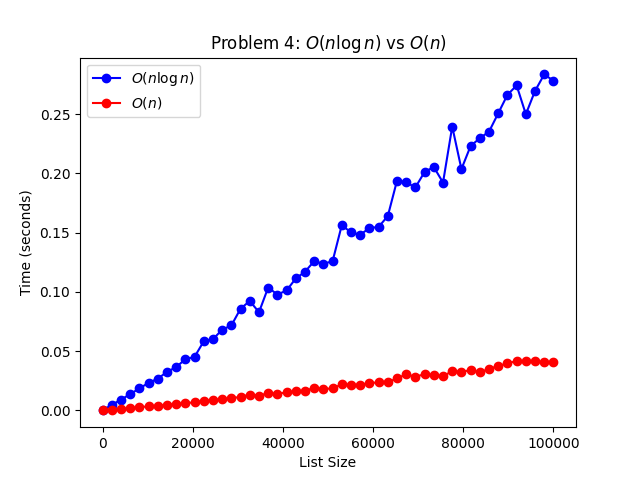
\includegraphics[width=0.5\textwidth]{figures/problem-4.png}
        \end{figure}
    \end{solution}
    
    Note that the mode can be negative. If $\delta_{i, j}$ is a mode of the list, then $-\delta_{i, j} = \delta_{j, i}$ will be a mode too. The input to the function will be one of these modes, which can be positive, negative, or 0.
\end{problem}

\newpage

%%%%%%%%%%%%%%%%%%%%%%%%%%%%%%%%%%%%%%%%%%%%%%%%%%%%%%%%%%%%%%%%%%%%%%%%%%%%%%%%
% Problem 5

\begin{problem}
  Eman baked some cookies for her friends, and asked Avital to help
  by distributing them among their friends. 
  Their group of friends is very close-knit, so they all live in a building 
  together, called ``The Building''.
  
  The architect of ``The Building'' designed 
  the property such that every floor is a very long corridor. To one side of 
  the corridor are all the apartments in that floor, with the distance between 
  every pair of consecutive doors being always the same.   
  The architect is not very fond of elevators, so to the other side of the 
  corridor, there is a pair of staircases in front of every apartment door,
  leading to all the floors in the building. 
  Apartments are labeled first by floor and then by index in the floor, hence 
  $apt_{(12,21)}$ is the 21st apartment in the 12 floor.

  Avital is not a big fan of walking, so as she delivers the cookies,
  she may give some extra cookies to her friends, and ask them to
  distribute them to some other friends. All the friends may subsequently
  divide their cookies and ask other friends to help with the deliveries too. 
  
  Avital wants to minimize everyone's total number of steps. Assume that the distance between an apartment $apt_{(f,i)}$ and $apt_{(f,i+1)}$ is the same as that between $apt_{(f,i)}$ and $apt_{(f+1,i)}$. 
  
  Assume the friends are distributed across $n$ apartments,
  where each apartment, including Eman's, has $p > n$ friends
  currently hanging out.
  Finally, assume that Avital starts at apartment $apt_{(1,1)}$,
  where Eman lives, and she can recruit some of the friends currently there.

  (\textit{20 points}) Design and implement an algorithm that given a list of apartments where the friends live, returns pairs $(a, b)$, where friends from apartment $a$ take the cookies to the friends from apartment $b$, that minimize the total number of steps. Your algorithm should run in $O(n^2 \log n)$.
  Describe your algorithm in the write-up and include your implementation in \texttt{problem\_5/p5.py}.

\begin{solution}
Please answer here.
\end{solution}
\end{problem}

\begin{challenge}
    \textbf{A closer look at Integer Multiplication}
    
    Given two $n$-bit integers (represented as a list of binary values, i.e. base 2), $x, y\in\{0,1\}^n$,
    implement three approaches to computing their product $x \cdot y$
    and perform an empirical performance analysis of the algorithms.

    (\textit{2 points}) The first approach will be a reference implementation. Compute the product by converting from their binary representation to an int, then multiplying. Please provide a brief description of your implementation here.
    
    \begin{solution}
        Please answer here.
    \end{solution}

    (\textit{5 points}) For the second approach,
    we would like you to implement the Karatsuba algorithm,
    described in section 5.5 of the Algorithm Design textbook.
    Please provide a brief description of your implementation here.

    \begin{solution}
        Please answer here.
    \end{solution}

    (\textit{10 points}) The final algorithm to implement is the Fast Fourier Transform (FFT), described in
    section 5.6 of the Algorithm Design textbook.
    Please provide a brief description of your implementation here.

    \begin{solution}
        Please answer here.
    \end{solution}


    (\textit{3 points}) Finally, provide an empirical performance analysis of the algorithms.
    Ensure that the analysis samples enough problem sizes (i.e. integer sizes $n$)
    such that the runtimes can be clearly differentiated.
    
    \begin{solution}
        Please answer here.
    \end{solution}

\end{challenge}

\end{document}
